% ---------------------------------------------------------------------------------------
\chapter{La transformaci\'on de Box-Cox}\label{chap4}

    La transformaci\'on de Box y Cox, conocida como Box-Cox, es una t\'ecnica de transformaci\'on no lineal que fue propuesta por George Box y David Cox en 1964 en su trabajo \textit{''An Analysis of Transformations''}\cite{boxcox64}. Cuenta la historia que el Profesor cox estaba visitando al doctor Box en Wisconsin, y decidieron que deberían escribir un artículo juntos dada la similitud de sus nombres, y que ambos eran británicos \cite{lane2003introduction}. 
    Muchos importantes resultados y t\'ecnicas en el an\'alisis estad\'istico de datos toman el supuesto de que los datos poseen una distribuc\'on normal, en los casos cuando este supuesto no se sostiene, una de las alternativas es transformar los datos para que se acerquen a una distribuci\'on normal. En este contexto la transformaci\'on de Box-Cox fue propuesta para convertir un conjunto de datos en una distribuci\'on que se asemeja a la normal, dejando una distribuci\'on con menos sesgo que es un poco m\'as sim\'etrica, esto suele ser determinado en base a un test de m\'axima verosimilitud, m\'as adeltante discutiremos el motivo de esto. La transformaci\'on de Box-Cox pertenece una familia de t\'ecnicas conocidas como transformaciones de potencia. Estas transformaciones buscan modificar los datos de entrada elev\'andolos a una potencia determinada, identificada por el par\'ametro $\lambda$.
    
    Box y Cox desarrollaron este m\'etodo con la intenci\'on de crear una t\'ecnica de transformaci\'on flexible que pudiera adaptarse a diversas distribuciones de datos, esto permite adaptar el coeficiente para funcionar en distintos contextos, y de nuestro interes particular es en el contexto de im\'agenes. En general la transformaci\'on solo es utilizada sobre vectones 1-dimensional. En 2020 Abbas Cheddad p\'ublico \textit{''On Box-Cox Transformation for Image Normality and Pattern Classification''}\cite{boxcoximg}, donde se discut\'io el coeficiente como un paso de preprocesamiento de im\'agenes, tanto para mejoramiento visual, como para mejorar el desempe\~no de algoritmos de clasificaci\'on. En este trabajo se propuso una nueva forma de aplicar la transformaci\'on, que consiste en utilizar el histograma de la imagen como proxy comprimido de la matriz de datos, y as\'i poder aplicar la transformaci\'on de forma r\'apida.
    
    En este cap\'itulo vamos a discutir la transformaci\'on de Box-Cox, presentaremos su definici\'on, y discutiremos el motivo de su uso. Luego vamos a discutir el trabajo de Cheddad\cite{boxcoximg}, y como este puede ser aplicado sobre im\'agenes. Finalmente discutiremos alternativas para calcular $\lambda$ sobre im\'agenes.
    
    \section{Definiciones}
    Para un $\lambda\in\R$ dado, la transformaci\'on de Box-Cox se define como:
    \begin{equation}\label{Box-Cox}
        y^{(\lambda)}= \begin{cases}\frac{y^{\lambda}-1}{\lambda} & (\lambda \neq 0) \\ \log y & (\lambda=0)\end{cases}
    \end{equation}
    
    $\forall y\in\R_{>0}$. En la pr\'actica los valores de $\lambda$ se restringen a un intervalo, normalmente $[-2,2]$ o $[-5,5]$, notemos adem\'as que en la practica se toma la segunda forma cuando $|\lambda|<0.01$\cite{boxcoximg}.
    
    Adem\'as existe una versi\'on para datos no positivos dada por:

    $$
    y^{(\lambda)}= \begin{cases}\frac{\left(y+\lambda_{2}\right)^{\lambda_{1}}-1}{\lambda_{1}} & \left(\lambda_{1} \neq 0\right), \\ \log \left(y+\lambda_{2}\right) & \left(\lambda_{1}=0\right) .\end{cases}
    $$

    Esta versi\'on es menos utilizada en la pr\'actica, dado que se suelen realizar otros pasos de preprocesamiento que dejan los datos entre 0 y 1.
    
    Cabe notar que Bicego y Baldo (2016)\cite{bicego2016} demostraron que, dado un vector $\textbf{y}=(y_1,\dots,y_n)\in\R^n_{>0}$, la transformaci\'on no cambia dado el orden de los elementos en el vector, por lo tanto al momento de aplicar la transformaci\'on sobre una imagen, o en general una matriz d-dimensional, se puede aplicar la cualquier ordenamiento sobre los datos, y luego aplicar la transformaci\'on sobre el vector unidimensional resultante. Dado esto tambi\'en cabe notar que al ser agn\'ostica con respecto al orden de los datos, la transformaci\'on no altera la relaci\'on espacial entre los datos.
    
    Como mencionamos anteriormente, el objetivo de la transformaci\'on es encontrar el valor de $\lambda$ que proporciona el mejor ajuste a una distribuci\'on normal. Para esto, Box y Cox proponen un criterio de m\'axima verosimilitud, el cual se define como:

    \begin{equation}
        \mathcal{L}(\lambda) \equiv-\frac{n}{2} \log \left[\frac{1}{n} \sum_{j=1}^{n}\left(x_{j}^{\lambda}-\overline{x^{\lambda}}\right)^{2}\right] +(\lambda-1) \sum_{j=1}^{n} \log x_{j}
    \end{equation}
    donde $\overline{x^{\lambda}}$ es el promedio muestral del vector transformado.

    La verosimilitud juega un papel crucial en el proceso de transformaci\'on de Box-Cox. En t\'erminos simples, la verosimilitud se refiere a la probabilidad de que un conjunto de datos observados se derive de una distribuci\'on estad\'istica particular. En este caso, la verosimilitud se utiliza para medir qu\'e tan bien una distribuci\'on normal se ajusta a los datos transformados para diferentes valores de $\lambda$. El valor de $\lambda$ que maximiza esta verosimilitud es el que se selecciona para la transformaci\'on.

    
    La transformaci\'on de Box-Cox persigue un objetivo esencial en el an\'alisis estad\'istico: garantizar el cumplimiento de los supuestos necesarios para la aplicaci\'on de modelos lineales. Esta garant\'ia posibilita el uso de t\'ecnicas de an\'alisis de varianza est\'andar en los datos transformados. En este sentido, Bicego y Bald\'o \cite{bicego2016} resaltan que esta transformaci\'on no altera el ordenamiento de los datos, manteniendo intacta la relaci\'on inherente entre ellos.

    Es importante aclarar, sin embargo, que no todos los conjuntos de datos pueden ser transformados de tal manera que resulten en una distribuci\'on normal perfecta. A pesar de esta limitaci\'on, Draper y Cox \cite{draper1969} argumentan que la transformaci\'on de potencia puede ser efectiva en muchos casos. Incluso en situaciones donde la transformaci\'on no logra una normalidad exacta, las estimaciones habituales del par\'ametro $\lambda$ pueden desempe\~nar un papel vital en la regularizaci\'on de los datos.

    Este proceso de regularizaci\'on conduce a una distribuci\'on que cumple con ciertos criterios deseables, como la simetr\'ia o la homocedasticidad. Esta \'ultima caracter\'istica, que se refiere a la constancia de la varianza a lo largo del conjunto de datos, es especialmente \'util en campos como el reconocimiento de patrones y el aprendizaje autom\'atico. Por ejemplo, en el an\'alisis discriminante lineal de Fisher, la homocedasticidad facilita la diferenciaci\'on entre diferentes clases de datos, potenciando la eficacia de este tipo de t\'ecnicas de aprendizaje autom\'atico.


    \section{Box-Cox sobre im\'agenes} 

    En su art\'iculo del 2020 \cite{boxcoximg}, Abbas Cheddad resalta una notable brecha en la aplicaci\'on de la transformaci\'on de Box-Cox a im\'agenes digitales. Seg\'un Cheddad, existe una carencia significativa de estudios en este \'ambito, destacando el trabajo de JD Lee en 2009 como una excepci\'on\cite{lee2009mr}. En el estudio de Lee, se present\'o un m\'etodo de segmentaci\'on para im\'agenes de resonancia magn\'etica cerebral a trav\'es de una t\'ecnica de transformaci\'on de distribuci\'on. En este enfoque, la transformaci\'on de Box-Cox se aplic\'o a las im\'agenes de resonancia magn\'etica cerebral para normalizar la distribuci\'on de intensidad de los p\'ixeles. Es relevante se\~nalar que, en este estudio, las im\'agenes se trataron como un vector de datos en lugar de una matriz, lo que implica un enfoque unidimensional en la manipulaci\'on y an\'alisis de la imagen.

    Cabe destacar que el proceso de aplicar la tranformaci\'on es iterativo, en el cual se ha de buscar un parametro $\lambda$, esto hace que aplicar esta la transformaci\'on en grandes bancos de im\'agenes sea demoroso. Una alternativa propuesta por A. Cheddad \cite{boxcoximg} es utilizar el histograma como proxy comprido de la matriz de datos, dado que este refleja la probabilidad estimada de que un pixel esa de un tono en particular. En lo que continua de la secci\'on discutiremos este m\'etodo.

    Como mencionamos en el cap\'itulo \ref{chap3}, podemos tratar una imagen como una funci\'on bidimensional $f(x,y)$, donde $x$ y $y$ son coordenadas espaciales, en este caso usaremos im\'agenes en el espacio de RGB, por lo que tenemos 
    
    $$
    f(x, y)=\{R(x, y), G(x, y), B(x, y)\}
    $$

    donde $(x, y)$ son las coordenadas en el espacio de pixeles que cumplen $x=0, \ldots X-1$, $y=0, \ldots Y-1$ y $(X, Y)$ son las dos dimensiones de la im\'agen. Ahora utilizaremos la transformaci\'on \ref{eq:grayscale}, para transformar la im\'agen a escala de grises de la siguiente forma

    \begin{equation*}
        \mathcal{F}(x, y)=0.299 R(x, y)+0.687 G(x, y)+0.114 B(x, y), 
    \end{equation*}

    que corresponde al canal de escala de grises como est\'a definido por el espacio de color $\mathrm{YC}_{\mathrm{b}} \mathrm{C}_{\mathrm{r}}$. Ya teniendo la im\'agen en escala de grises, i.e., en forma de matriz de $XxY$, podemos aplicar la formula \ref{Box-Cox} luego de aplicar alguna operaci\'on que tranforme la matriz a un vector de los mismos valores. Recordemos que los particulares de esta transformaci\'on no son de importancia, m\'as all\'a de que la transformaci\'on debe ser reversible, dado que la transformaci\'on de Box-Cox es agn\'ostica al orden del vector.

    Ahora nos hace falta elegir un $\lambda$ para aplicar la transformaci\'on, discutiremos la elecci\'on de este en la siguiente secci\'on, pero asumiento que ya tenemos uno seleccionado, podemos aplicar Box-Cox sobre la imagen. Para esto debemos tomar en cuenta que nuestra imagen, posterior al paso a blanco y negro, esta constituida por valores entre $0$ y $255$, pero la transformaci\'on de Box-Cox no esta definida para valores no positivos, por lo tanto debemos trasladar los datos para que esten en el rango $[1,256]$, y luego aplicar la transformaci\'on. Adem\'as, para facilidad de calculo los valores son llevados al intervalo $[\frac{1}{256},1]$.

    Pero esto nos entrega un \'ultimo problema, posterios a la transformaci\'on podemos obtener valores que est\'en por encima de 1, por lo tanto debemos normalizar los datos para que esten en el intervalo $[0,1]$. Para esto definimos Box-Cox para im\'agenes o BCI como:

    \begin{defn}[Box-Cox para im\'agenes]

        Sea $\mathcal{F}^{\lambda_{\cdot}(x, y)}$ las im\'agen transformada para alg\'un $\lambda_\cdot$ seleccionado, entonces definimos BCI como:

    \begin{equation}
        BCI = \frac{\left(\mathcal{F}^{\lambda_{\cdot}}(x, y) - \min\left(\mathcal{F}^{\lambda_{\cdot}}(x, y)\right)\right)}{\left(\max\left(\mathcal{F}^{\lambda_{\cdot}}(x, y)\right) - \min\left(\mathcal{F}^{\lambda_{\cdot}}(x, y)\right)\right)}
    \end{equation}
        
        
    \end{defn}

    Notemos que este \'ultimo paso se realiza para que los datos esten entre 0 y 1, y as\'i poder ser representados en una imagen.
    
    \subsection{Ejemplos}
    
    En las siguientes figuras \ref{fig:all_lambda_1} \ref{fig:all_lambda_2} se puede ver un ejemplo de la transformaci\'on aplicada sobre dos im\'agenes, en particular la im\'agen 1 y 3 del banco, para distintos valores de $\lambda$ ubicados en el intervalo $[-2,5]$, estos valores fueron selecionados pues es donde la transformaci\'on es m\'as efectiva.

    Es claro a simple vista que valores m\'as bajos de $\lambda$ producen im\'agenes m\'as ''claras'', hasta el punto en que la imagen es completamente blanca. Por otro lado, valores m\'as altos de $\lambda$ producen im\'agenes m\'as ''oscuras'', pero en general podemos ver que el rango \'util para im\'agenes es $[-0.25,4]$, puesto que valores m\'as altos o m\'as bajos producen im\'agenes casi indistinguibles. 

    Esto es f\'acil de corroborar al momento de analizar los histogramas, que podemos ver en las figuras \ref{fig:img_bci_hist_1} y \ref{fig:img_bci_hist_2} 

    \begin{figure}
        \centering
        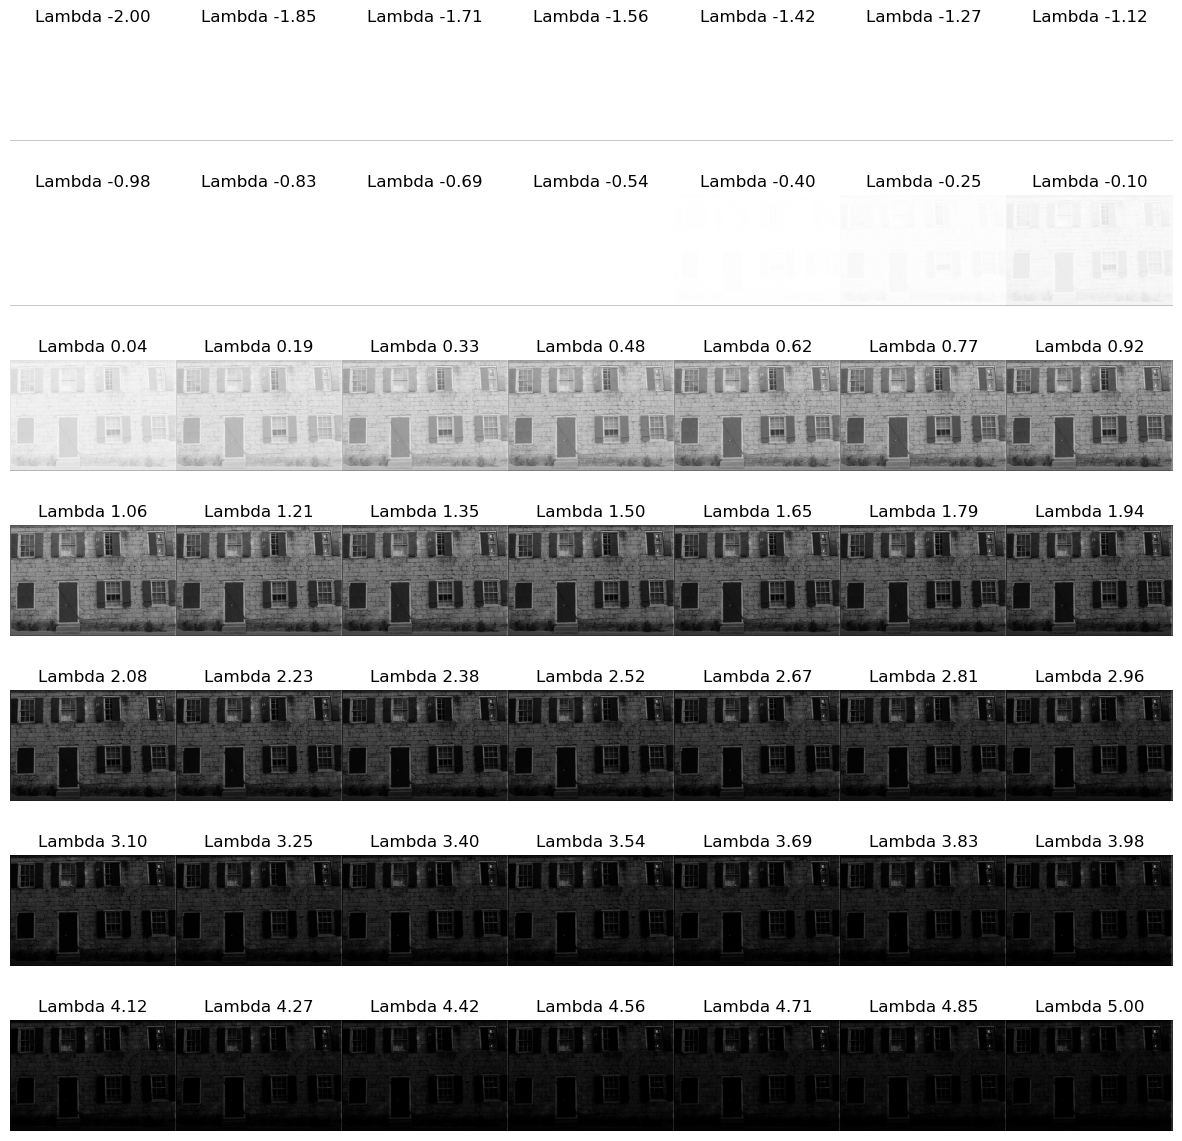
\includegraphics[width=\textwidth]{all_lambda_1.png}
        \caption{Transformaciones de la im\'agen 1.}
        \label{fig:all_lambda_1}
    \end{figure}

    \begin{figure}
        \centering
        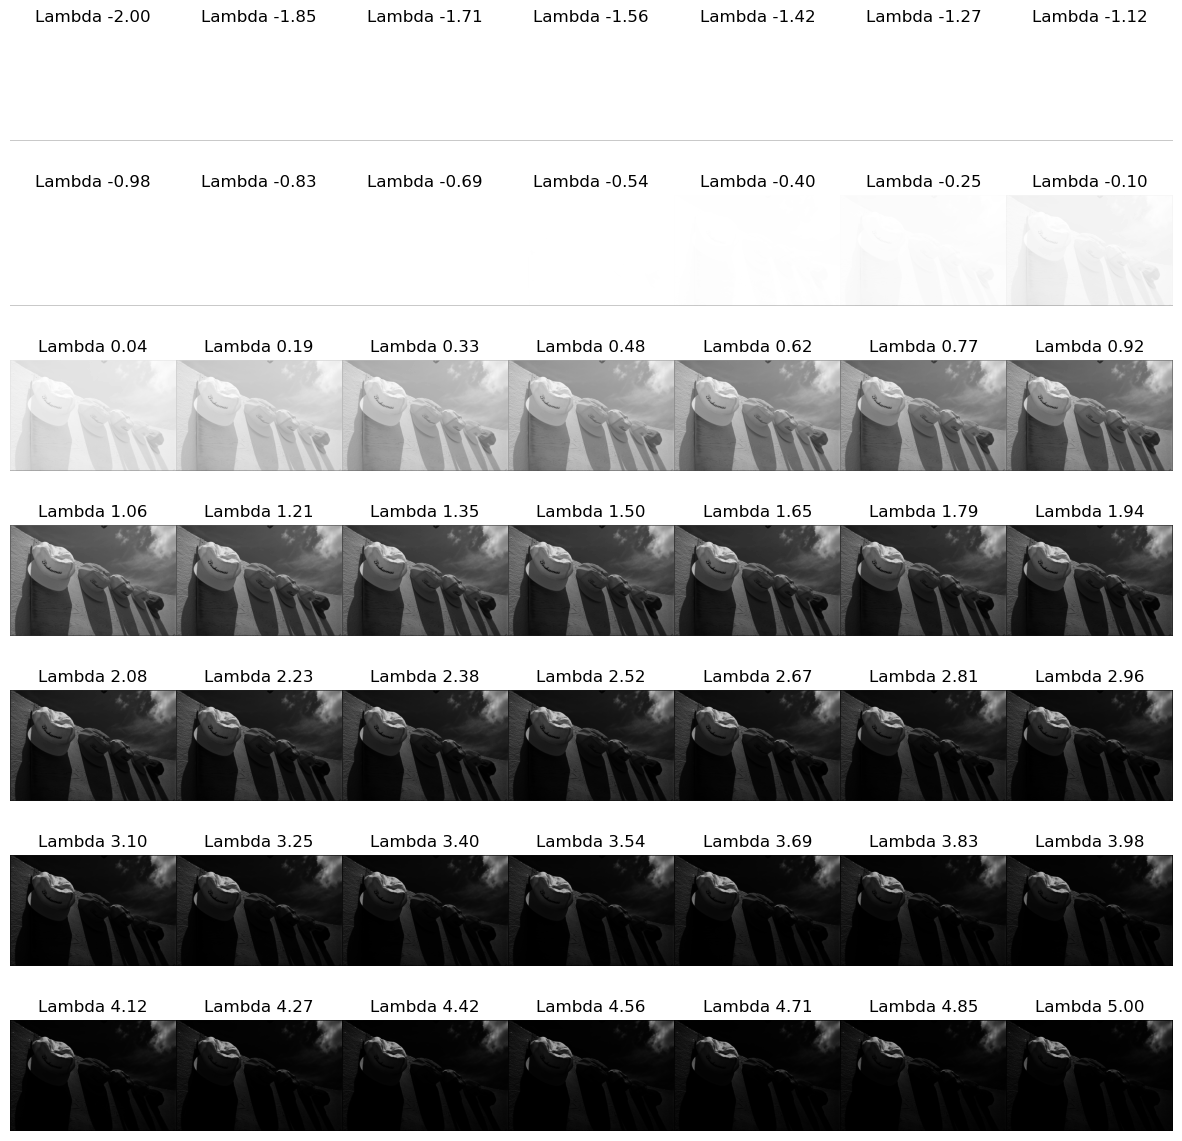
\includegraphics[width=\textwidth]{all_lambda_3.png}
        \caption{Transformaciones de la im\'agen 3.}
        \label{fig:all_lambda_2}
    \end{figure}

    \begin{figure}
        \centering
        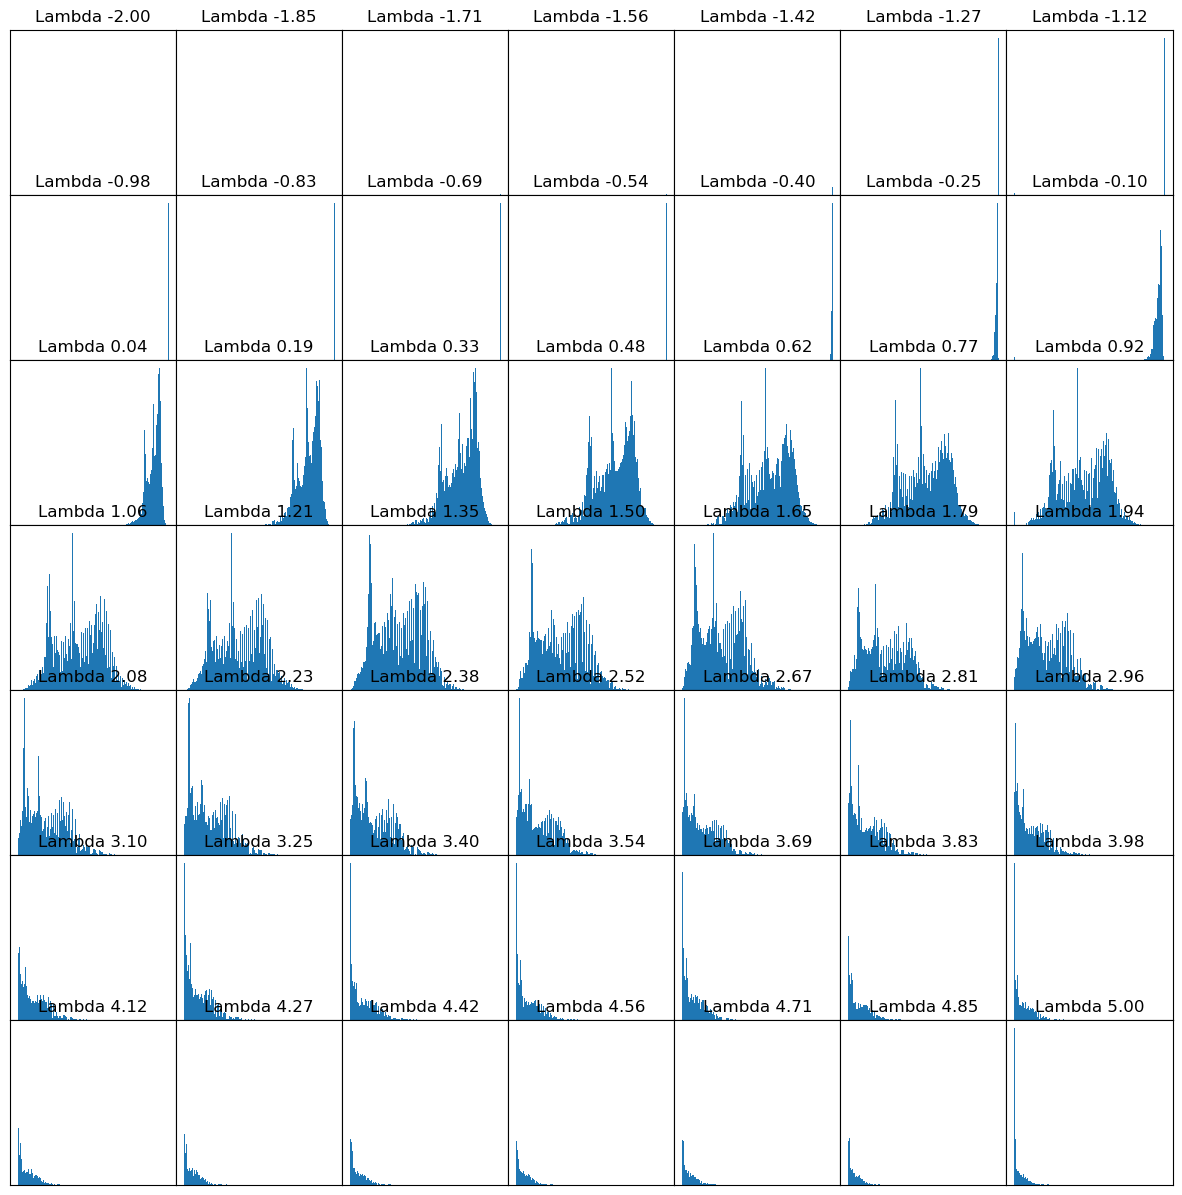
\includegraphics[width=\textwidth]{all_lambda_hist_1.png}
        \caption{Histograma de las transformaciones de la im\'agen 1.}
        \label{fig:img_bci_hist_1}
    \end{figure}

    \begin{figure}
        \centering
        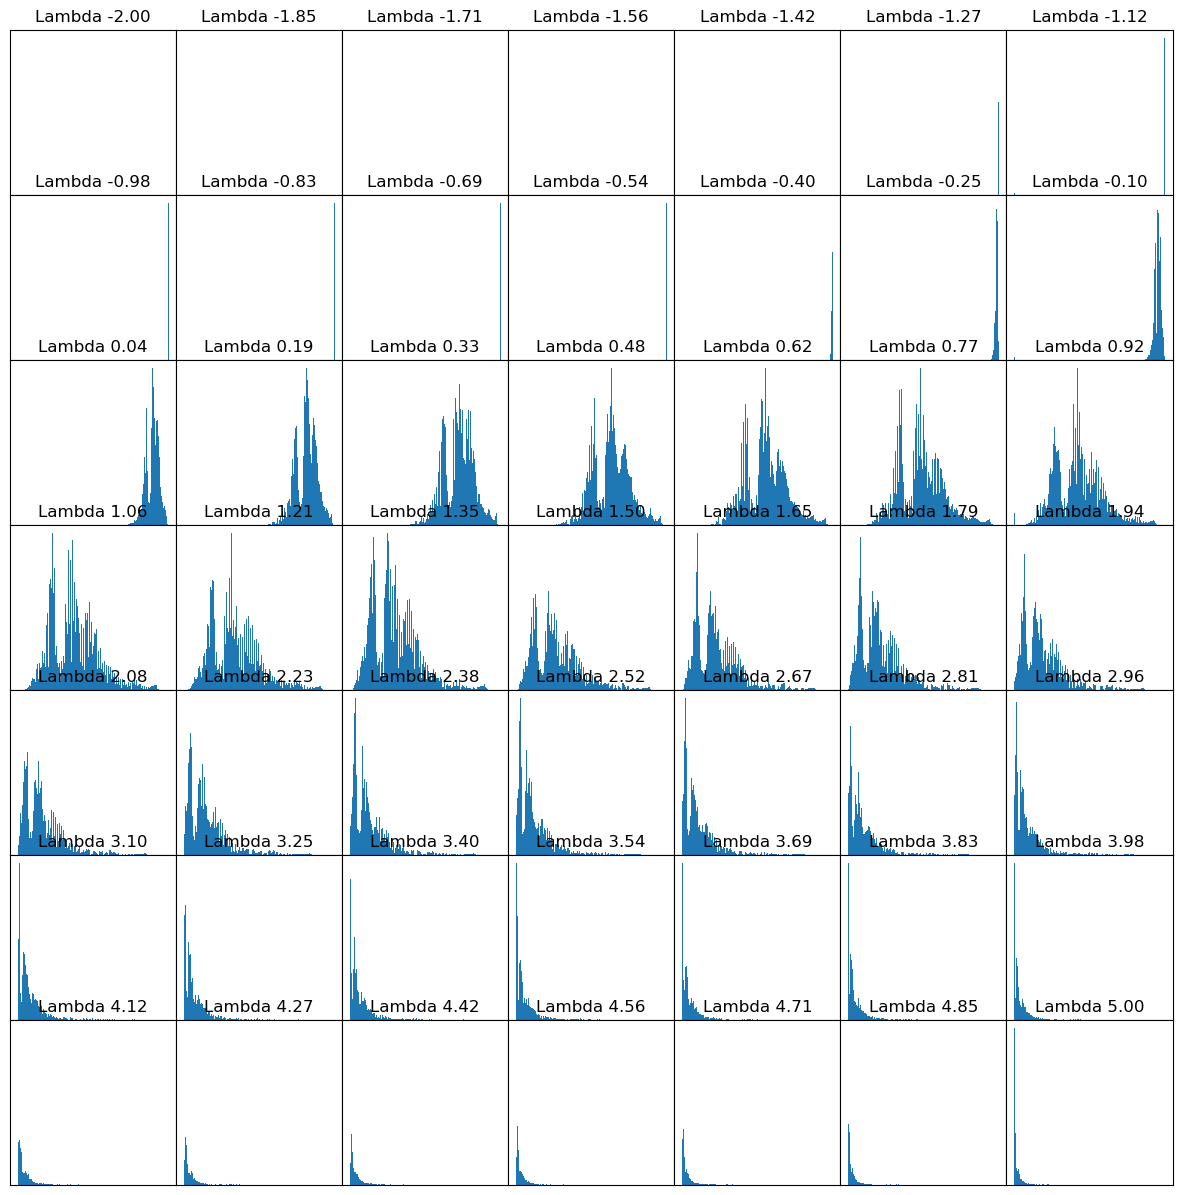
\includegraphics[width=\textwidth]{all_lambda_hist_3.png}
        \caption{Histograma de las transformaciones de la im\'agen 2.}
        \label{fig:img_bci_hist_2}
    \end{figure}

    Podemos ver como la transformacion ''mueve'' los datos hac\'ia la izquierda mientras m\'as alto es el valor de $\lambda$, adem\'as mientras m\'as extremo es este valor, los datos se ven m\'as comprimidos. Esto confirma la idea de que hay un rango de valores los cuales son los m\'as \'utiles al momento de aplicar la transformaci\'on sobre ima\'agenes



    \section[Propuestas de lambda]{Propuestas de $\lambda$ para im\'agenes.}\label{}


    Ya teniendo la im\'agen como un vector, debemos decidir un $\lambda$ el cual usaremos para realizar la transformaci\'on. En esta secci\'on revisaremos los dos m\'etodos utilizados en la literatura, junto con otro que se propone en este trabajo. Luego en el siguiente cap\'itulo compararemos los resultados de estos procedimientos utilizando los m\'etodos de comparaci\'on de im\'agenes definidos en el cap\'itulo \ref{chap2}.


    \subsection{Box-Cox sobre datos completos}

    Este es el m\'etodo utilizado por Lee et. al. \cite{lee2009mr}, y consiste en aplicar la transformaci\'on sobre los datos completos, i.e., transformar la matriz a vector de alguna forma y luego aplicar verosimilitud para determnar el lambda. Notemos que la forma en la que la matriz sea transformada a vector no es de particular importancia, dado que la transformaci\'on es agn\'ostica con respecto al orden de los datos. 

    \begin{defn}\label{lambda_full}
        Sea $\mathcal{F}(x, y)\in\mathcal{M}_{n\times m}$ la imagen en escala de grises, y $\mathcal{F}^{\prime}(i)\in\R^{n\times m}$ el vector de datos, entonces definimos $\lambda_{full}$ como el valor de $\lambda$ que maximiza la verosimilitud de los datos completos, i.e., $\mathcal{F}^{\prime}(i)$.
    \end{defn}
    
    Este m\'etodo es el m\'as utilizado en la literatura, pero como mencionamos anteriormente, este no toma en cuenta la correlaci\'on espacial de los datos, y por lo tanto no es el m\'as adecuado para im\'agenes. 



    \subsection{Box Cox sobre histograma}

    En base a esto definimos la funci\'on de probabilidad de im\'agen, i.e., el histograma como:
    
    $$\chi(i)= \# \{\mathcal{F}(x,y)=i | x\in[0,X-1], y\in[0,Y-1] \}$$ 

    donde $i$ es el nivel de gris. Notemos que, para nuestro caso y en general, i es un entero entre 0 y 255, puesto que mayormente trabajamos con im\'agenes en 8-bits. Pero este tambien puede ser un valor real entre 0 y 1, o un valor entero entre 0 y $N\in\Nset$, dependiendo de la cantidad de bits que se utilicen para representar la imagen. Lo definimos cómo:

    \begin{defn}\label{lambda_hist}
        Sea $\mathcal{F}(x, y)\in\mathcal{M}_{n\times m}$ la imagen en escala de grises, y $\chi(i)\in\R^{256}$ el vector de histograma, entonces definimos $\lambda_{\chi}$ como el valor de $\lambda$ que maximiza la verosimilitud del vector histograma, i.e., $\chi(i)$.
    \end{defn}
    
    Fue obserado por Cheddad que estos dos m\'etodos ya definidos no coinciden (de hecho la correlaci\'on obervada en su experimento es $\rho=-0.3022$).

    \subsection{Box-Cox Grilla}

    En este m\'etodo utilizamos una grilla sobre la imagen, luego calculamos el $\lambda$ para cada subimagen, y finalmente calculamos el promedio de estos. Este m\'etodo busca tomar ventaja de la correlaci\'on espacial de los datos, y as\'i obtener un mejor valor de $\lambda$, el cual sea representativo de la imagen completa.

    
    \begin{defn}\label{lambda_grid}
        Sea $\mathcal{F}(x, y)\in\mathcal{M}_{n\times m}$ la imagen en escala de grises, y sea $r \in \mathcal{N} $ una resoluci\'on dada, definimos $\mathcal{F}_{i,j}(x, y)\in\mathcal{M}_{r\times r}$ como la $i,j$-ésima subimagen, con $i\in[0,\lfloor\frac{n}{r}\rfloor]$ y $i\in[0,\lfloor\frac{m}{r}\rfloor]$ las coordenadas de la subimagen.
        
        Ahora, para cada una de estas subim\'agenes definimos $\lambda^{i,j}_full$, como el valor $\lambda$ resultado de usar el m\'etodo definido en \ref{lambda_full} en la subim\'agen.

        Por ultimo, definimos $\lambda_{grid}$ como:
        
        $$
        \lambda_{grid} := \frac{\sum_{i,j} \lambda^{i,j}_full}{\lfloor\frac{n}{r}\rfloor\lfloor\frac{m}{r}\rfloor}.
        $$
    \end{defn}
    
        Durante este trabajo se uso una grilla de tama\~no $10x10$. Notemos adem\'as que para evitar problemas en el borde de la imagen, dejamos de lado las subim\'agenes que no tienen el tama\~no completo.

    Ahora en la siguiente figura \ref{fig:img_bci_all} podemos ver las transformaciones de cada una de est\'as im\'agenes, junto con el $\lambda$ seleccionado para cada una. Las transformaciones del resto de las im\'agenes pueden ser encontradas en el Ap\'endice \ref{appA}.


    \begin{figure}[H]
        \centering
        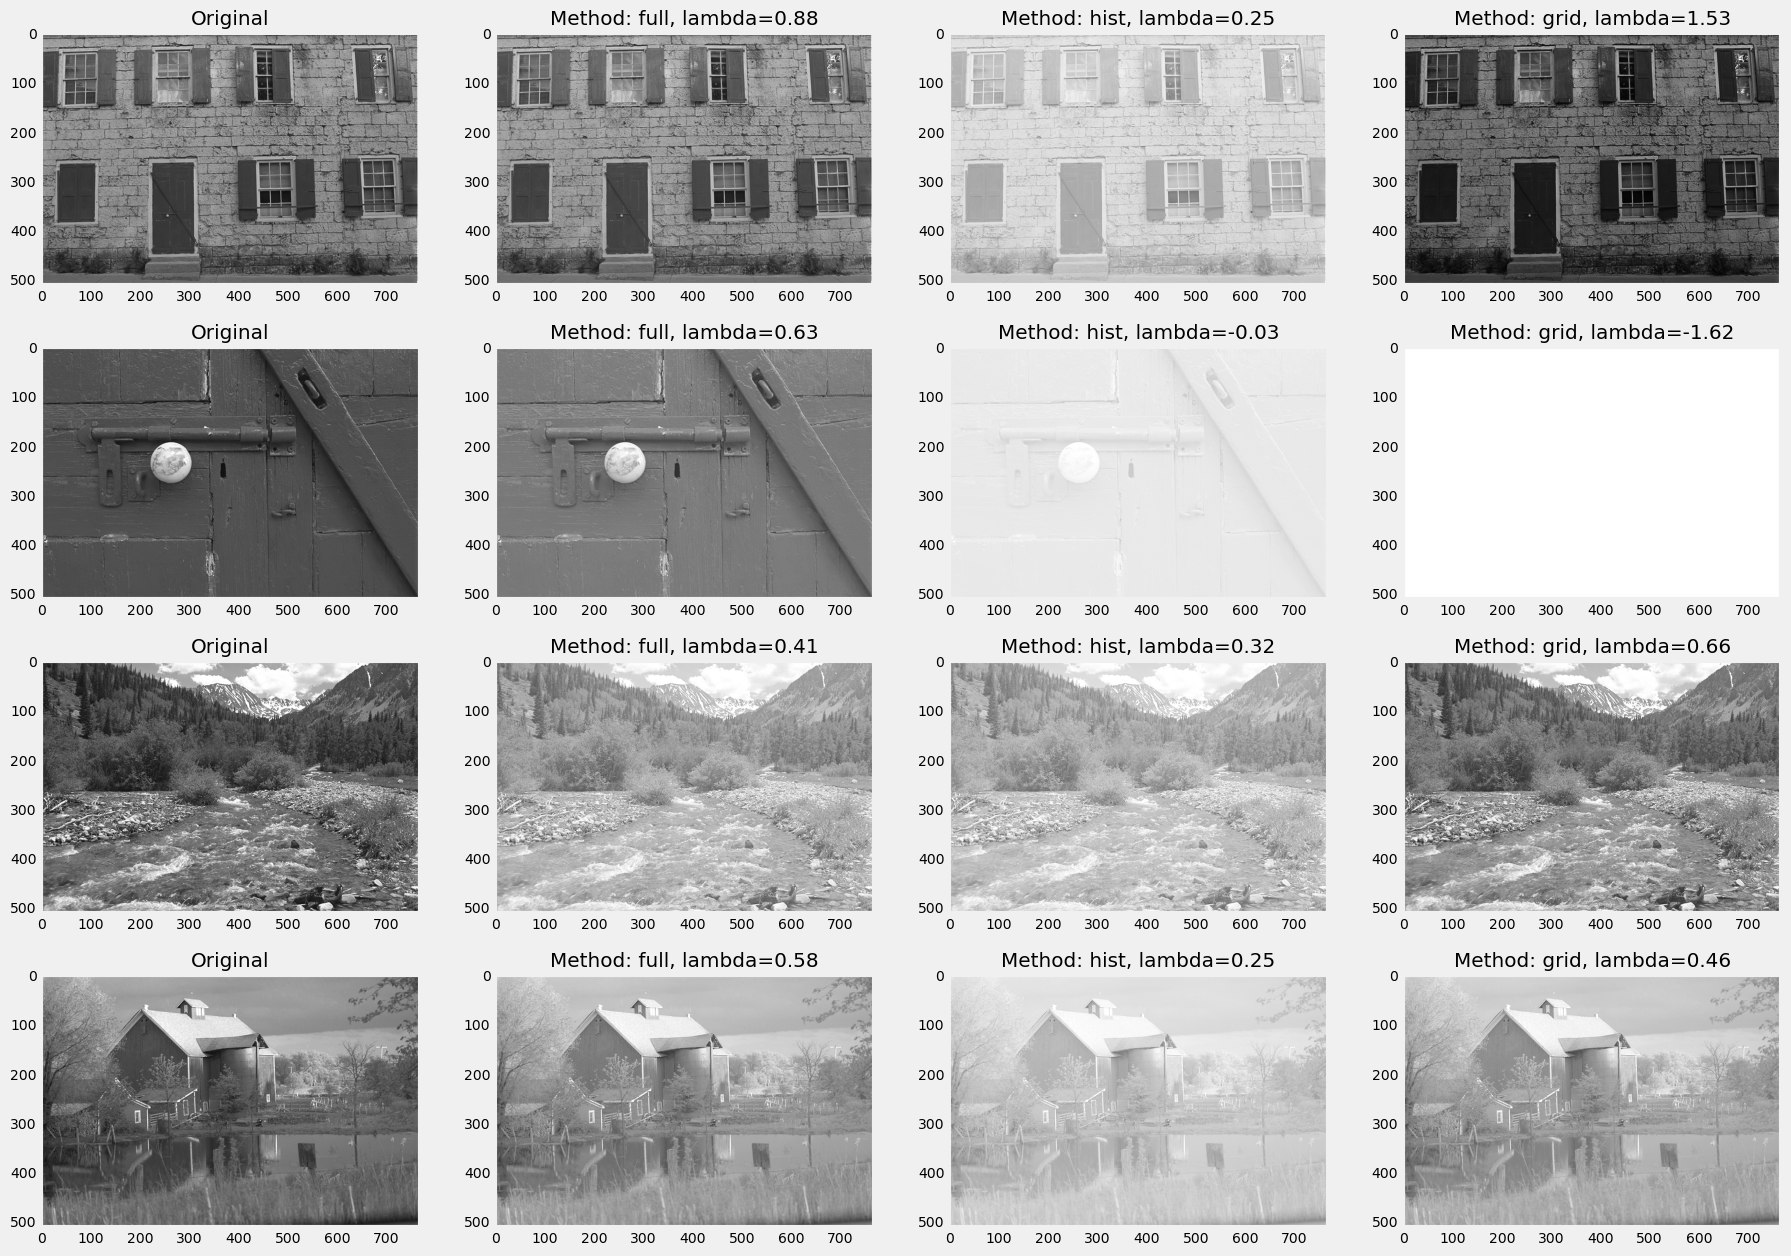
\includegraphics[width=\textwidth]{img_bci_all.png}
        \caption{Transformaciones de la im\'agen 1, 2, 13, y 22. De izquierda a derecha, im\'agen original, m\'etodo de datos completos, m\'etodo de histograma, y m\'etodo de grilla.}
        \label{fig:img_bci_all}
    \end{figure}


    Lo primero que notamos al ver l\'as im\'agenes es que el efecto que cada m\'etodo tiene en la imagen es distinto, m\'as abajo discutiremos los particulares de cada uno, pero de buenas a primeras es claro que el m\'etodo de grilla tiene un comportamiento m\'as err\'atico que los otros dos m\'etodos, mientras que el m\'etodo de histograma y el m\'etodo de datos completos tienen un comportamiento m\'as estable.

    No es extra\~no que la composici\'on de cada im\'age    n afecta el valor de $\lambda$ seleccionado, pero parece que esto es m\'as pronunciado en el m\'etodo de grilla, que en los otros dos m\'etodos. Esto se debe a que el m\'etodo de grilla es susceptible a grandes secciones de la im\'agen que tienen un bajo contraste, i.e. secciones de la im\'agen con valores de brillo sismilares, lo que genera que el valor de $\lambda$ se dispare. 

    Notemos, por otro lado, que el m\'etodo de histograma y el m\'etodo de datos completos tienen un comportamiento m\'as estable. Pero de la misma forma que Cheddad \cite{boxcoximg}, notamos que estos m\'etodos tampoco suelen coincidir, y que el m\'etodo de histograma suele seleccionar valores m\'as bajos de $\lambda$ que el m\'etodo de datos completos.
    
    Ahora, veamos como se comportan $\lambda$ en todo el banco de im\'agenes, separado por m\'etodo. Cabe mencionar que a pesar de que  en la primera secci\'on de este cap\'itulo hablamos de que la transformaci\'on de Box-Cox es utilizada para $\lambda\in[-5,5]$, dejamos sin l\'imite los valores de este para ver los resultados que obteniamos con los distintos m\'etodos.

    \begin{figure}[H]
        \centering
        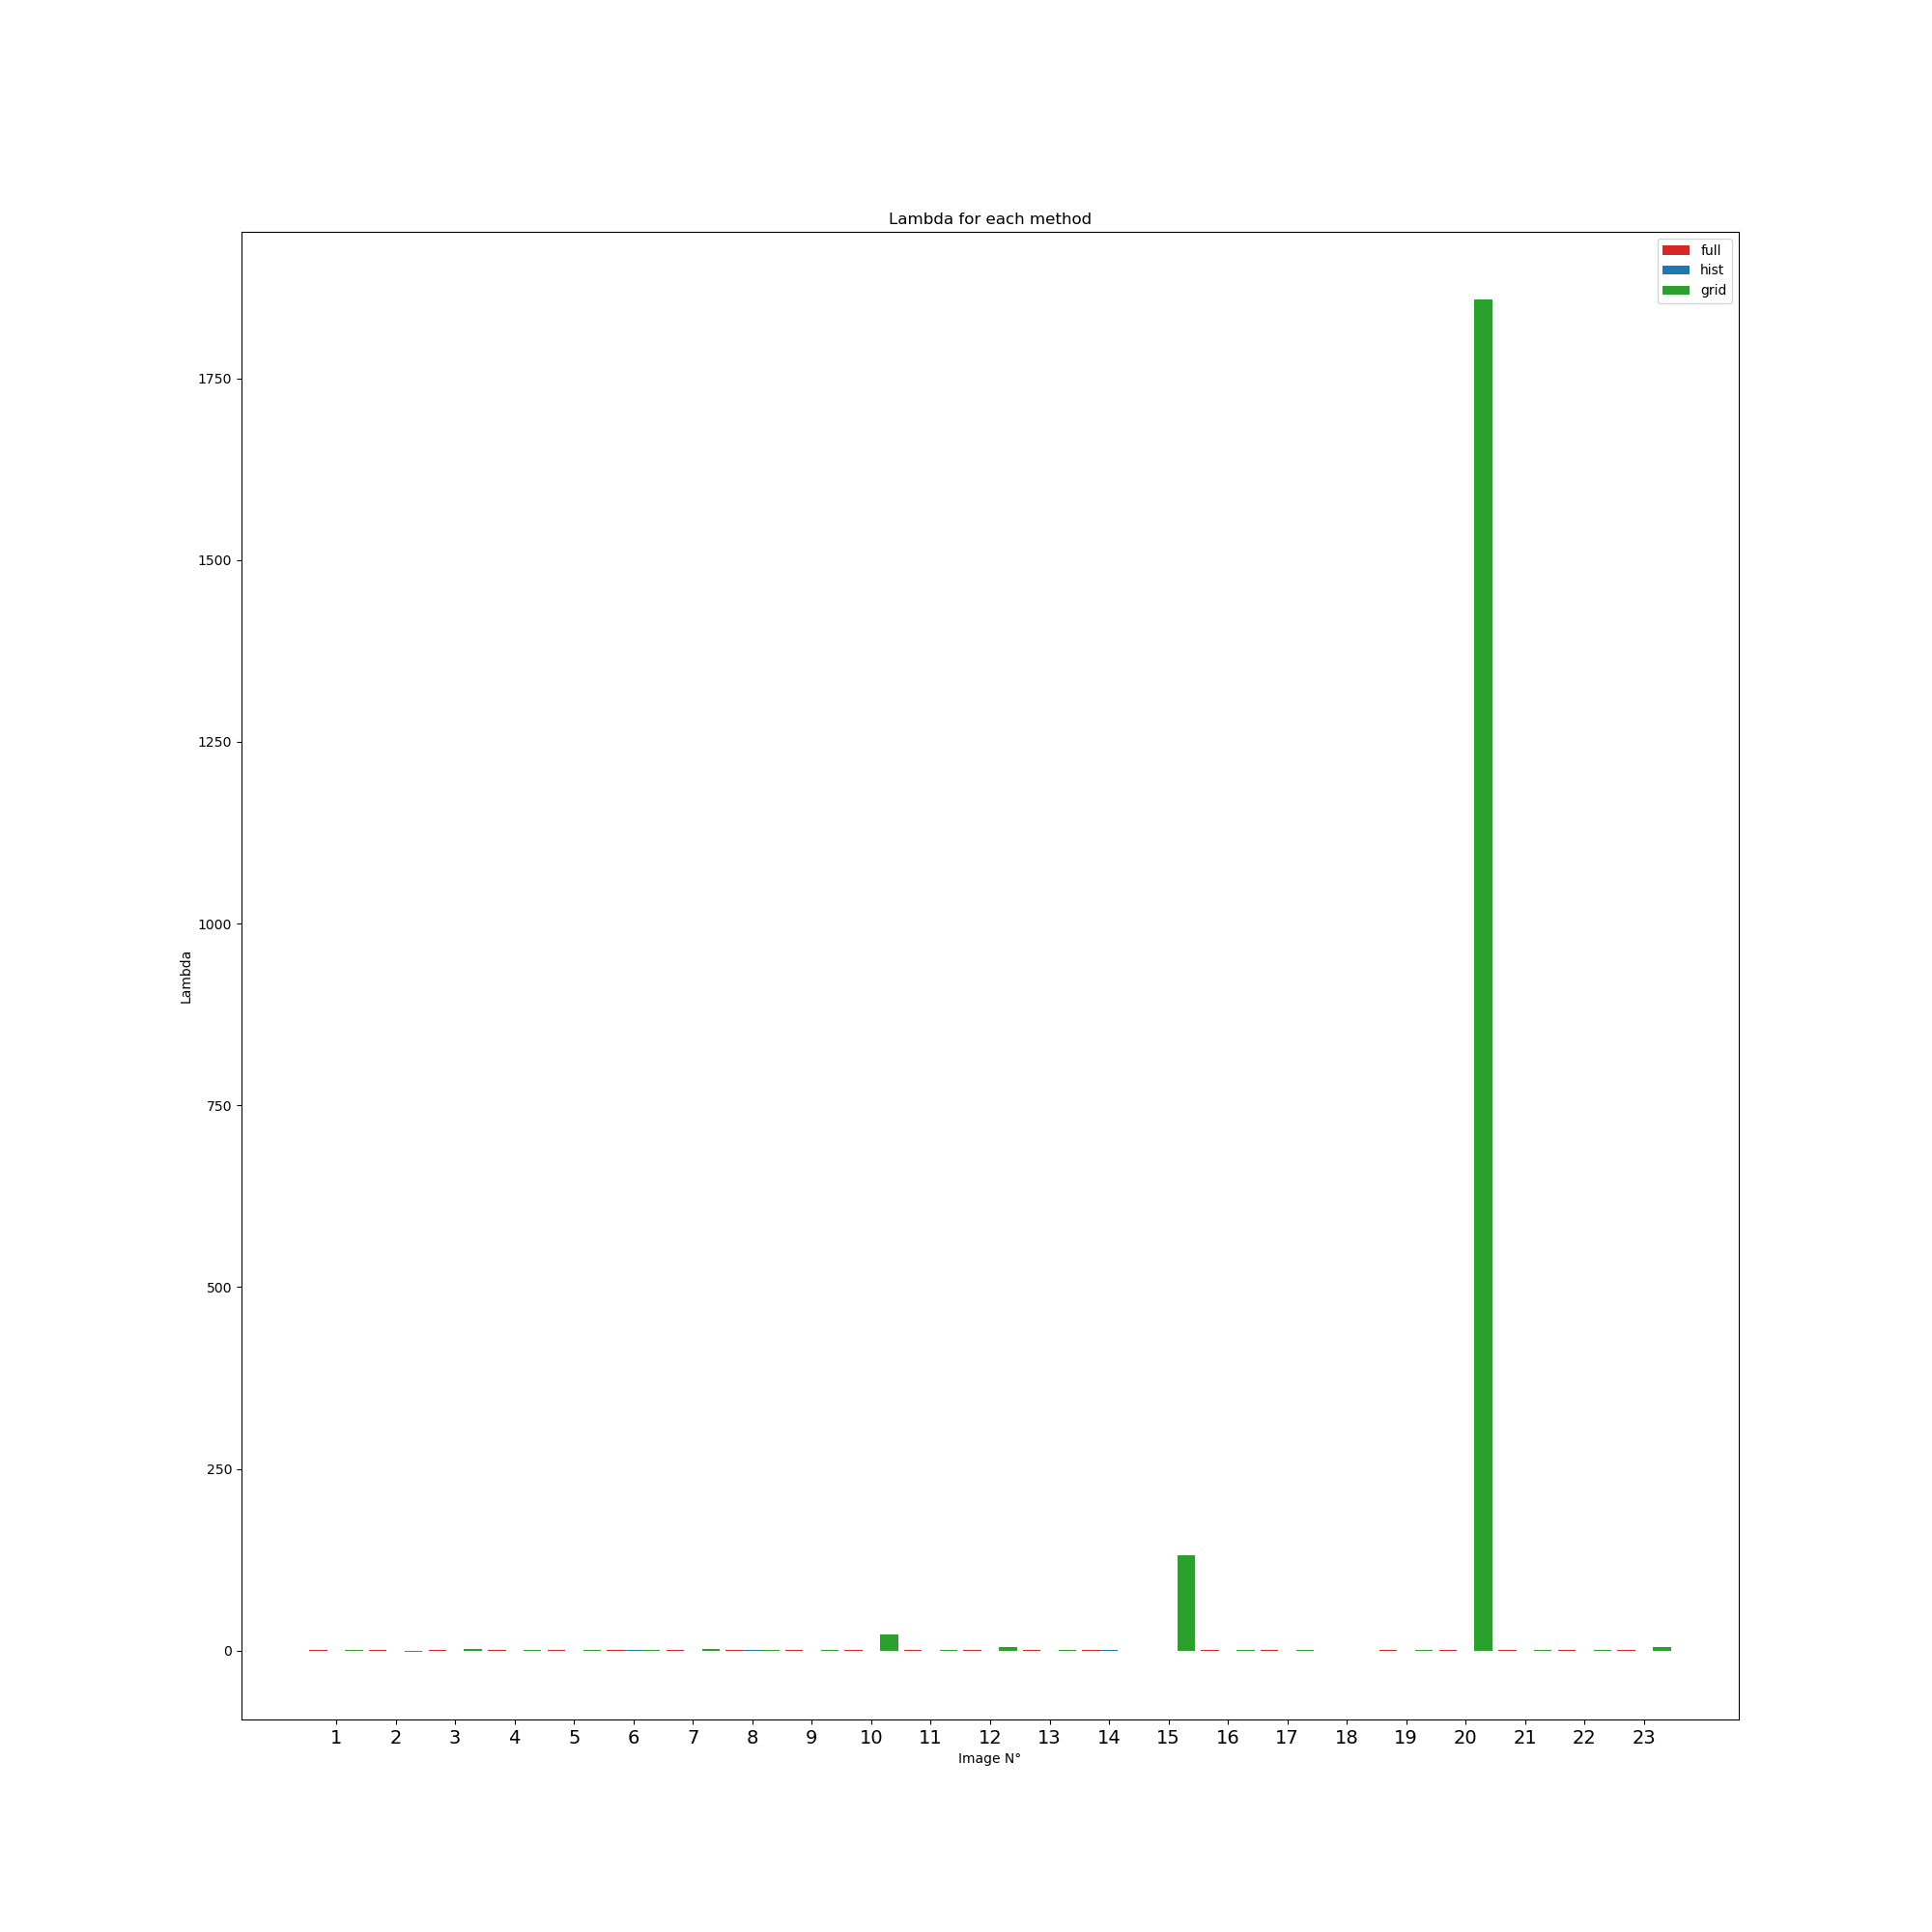
\includegraphics[width=0.6\textwidth]{lambda_noclip.png}
        \caption{Valores de $\lambda$ para todo el banco de im\'agenes. verde es el m\'etodo de grilla, azul es el m\'etodo de histograma, y rojo es el m\'etodo de datos completos.}
        \label{fig:lambda_noclip}
    \end{figure}

    Lo primero que notamos es que el m\'etodo de grilla tiene un comportamiento mucho m\'as err\'atico que los otros dos m\'etodos, en particular suele dispararse a valores extremadamente altos de $\lambda$. Notemos que las im\'agenes cuyo $\lambda$ se dispara son las im\'agenes 10, 15, 20, y 24, las cuales podemos ver a continuaci\'on en la figura \ref{fig:img_bci_10_15_20}

    \begin{figure}[H]
        \centering
        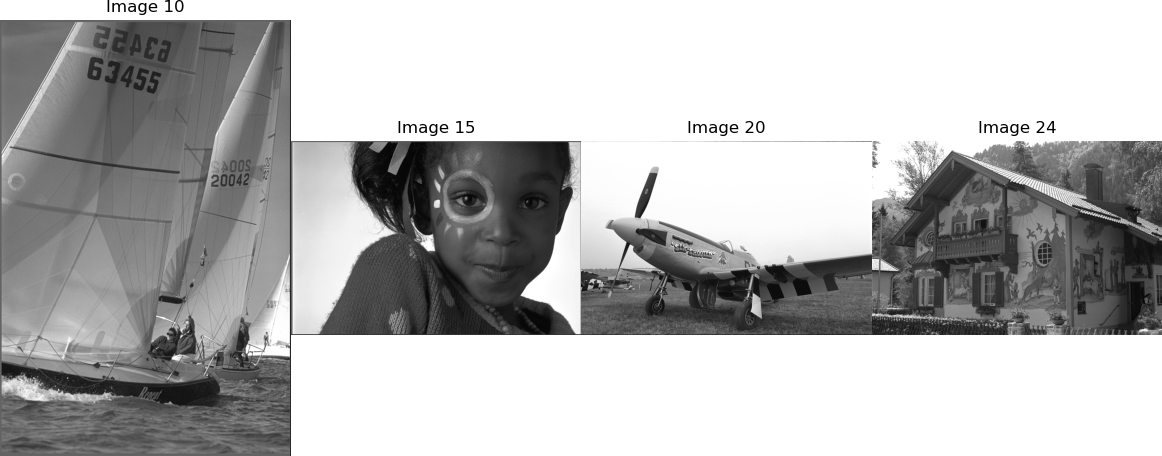
\includegraphics[width=0.9\textwidth]{img_ex_10_15_20_24.png}
        \caption{Im\'agenes 10, 15, 20, y 24.}
        \label{fig:img_bci_10_15_20}
    \end{figure}

    Lo que estas im\'agenes tienen en com\'un es que contienen grandes secciones de color similar, o bajo contraste, lo que genera que, al momento de hacer la grilla muchas secciones se ven ''planas'', esto genera que el valor de $\lambda$ se dispare. Ahora, vamos a cortar los valores en $5$ para poder ver mejor el comportamiento de $\lambda$ en el resto de las im\'agenes.

    \begin{figure}[H]
        \centering
        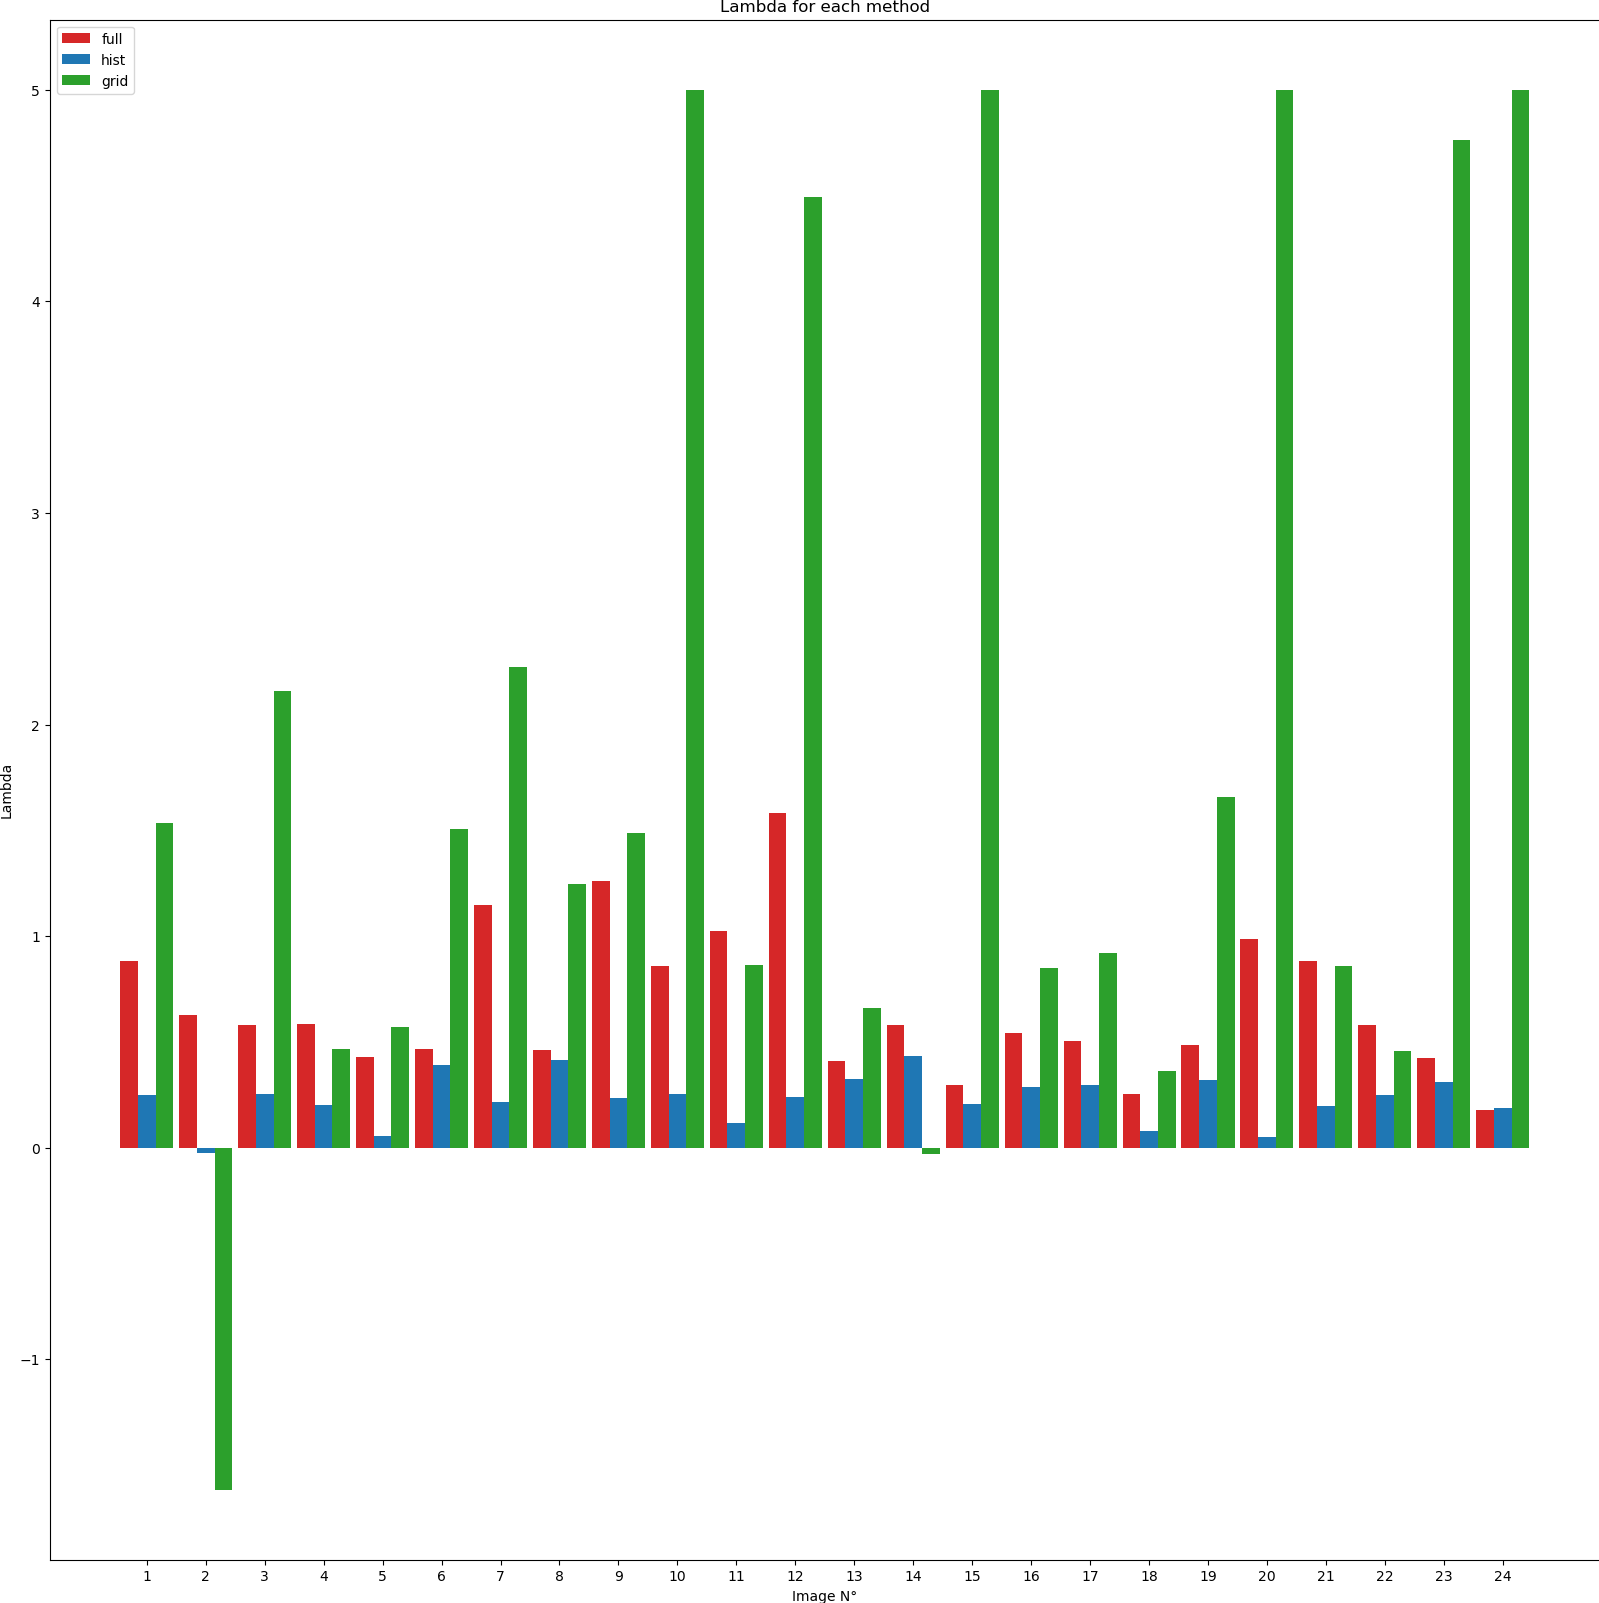
\includegraphics[width=0.7\textwidth]{lambda_clip.png}
        \caption{Valores de $\lambda$ para todo el banco de im\'agenes, cortado en 5. verde es el m\'etodo de grilla, azul es histograma, y rojo es datos completos}
        \label{fig:lambda_clip}
    \end{figure}

    Aqu\'i ya podemos ver el comportamiento de los $\lambda$ con m\'as detalle, y notamos que el m\'etodo de grilla sigue teniendo un comportamiento m\'as err\'atico, es Incluso el \'unico m\'etodo que nos entreg\'o un valor negativo para $\lambda$. Esto ocurrio en la im\'agen numero 2, la cual podemos ver en la figura \ref{fig:img_bci_all}. Por otro lado, el m\'etodo de histograma y el m\'etodo de datos completos tienen un comportamiento m\'as estable. 
    
    Notemos que el m\'etodo de histograma nos entrega valores m\'as bajos de $\lambda$ que el m\'etodo de datos completos, pero esto no es siempre cierto, y en particular para el banco de im\'agenes que estamos utilizando, ocurre lo contrario en una oportunidad, la im\'agen n\'umero 24.

    Ahora, podemos revisar que valores tuvieron las correlaciones de pearson entre los distintos m\'etodos de selecci\'on de $\lambda$.


    \begin{table}[H]
        \centering
        \begin{tabular}{|l|l|l|l|}
            \hline
            M\'etodo 1 & M\'etodo 2 & Pearson $\rho$ & Valor P \\ \hline
            Completo                  & Histograma                & -0.1305   & 0.5431  \\ 
            Completo                  & Grilla                    & 0.1384    & 0.5191  \\ 
            Histograma                & Grilla                    & -0.3467   & 0.0968  \\ \hline
        \end{tabular}
    \end{table}

    De aqu\'i podemos destacar que el valor de la correlaci\'on encontrados por Cheddad \cite{boxcoximg} entre el m\'etodo completo y el del histograma es de $\rho=-0.3022$, que es similar al encontrado en nuestros experimentos. Otro resultado interesante es que la correlaci\'on con m\'agnitud m\'as alta es entre el m\'etodo del histograma y el de la grilla, lo que sugiere una mayor relaci\'on entre estos, pero a\'un as\'i  no es un valor muy alto.

